\documentclass[conference]{IEEEtran}
\IEEEoverridecommandlockouts
\hbadness=10000
\vbadness=10000
\hfuzz=100pt
\vfuzz=100pt

\usepackage[utf8]{inputenc}
\usepackage[T1]{fontenc}
\usepackage{amsmath,amssymb}
\usepackage{graphicx}
\usepackage{booktabs} 
\usepackage{placeins}
\usepackage[hidelinks]{hyperref}
\usepackage{microtype} % Improves typography and fixes most underfull/overfull hboxes
\usepackage{tabularx}  % For flexible width tables
\usepackage{balance}   % To balance bottom columns on the last page


\newcommand{\name}{TabICLv2}
\newcommand{\TFcol}{\mathrm{TF}_{\mathrm{col}}}
\newcommand{\TFrow}{\mathrm{TF}_{\mathrm{row}}}
\newcommand{\TFicl}{\mathrm{TF}_{\mathrm{icl}}}
\title{Beyond Gradient Boosting: TabICL for Cart-to-Purchase Conversion Prediction in E-commerce}

\author{%
\IEEEauthorblockN{Le Hoai Thanh Quang}
\IEEEauthorblockA{FPT University, Ho Chi Minh City, Vietnam}
\and
\IEEEauthorblockN{Thai Viet Nam}
\IEEEauthorblockA{FPT University, Ho Chi Minh City, Vietnam}
\and
\IEEEauthorblockN{Nguyen Tai Phuc}
\IEEEauthorblockA{FPT University, Ho Chi Minh City, Vietnam}
\and
\IEEEauthorblockN{Nguyen Quoc Ky}
\IEEEauthorblockA{FPT University, Ho Chi Minh City, Vietnam}
}


\begin{document}

\maketitle
\begingroup
\renewcommand{\thefootnote}{}
\footnotetext{\raggedright\textbf{Code repository:}\\[-1pt]\url{https://github.com/TQuang122/Cart-to-Purchase-Conversion-Prediction}}
\endgroup

\begin{abstract}
Predicting cart-to-purchase conversion is a pivotal task in e-commerce, enabling platforms to identify high-intent users and orchestrate personalized interventions. Although Gradient-Boosted Decision Trees (GBDTs), notably XGBoost, have historically dominated tabular classification in industrial applications, they require extensive feature engineering, hyperparameter tuning, and frequent retraining cycles. Tabular foundation models, particularly those employing In-Context Learning (ICL), offer a scalable alternative where models generate predictions from training instances as context without iterative parameter updates. This paper presents a systematic empirical comparison of XGBoost and TabICL---a tabular foundation model pretrained on synthetic datasets---for cart-to-purchase conversion on a large-scale e-commerce behavioral dataset comprising over 285 million user interaction events. We formulate the task as conditional binary classification following an add-to-cart event and evaluate both models on a shared feature space via an end-to-end MLOps pipeline. Our results show that TabICL achieves competitive AUC-ROC performance on datasets exceeding 50,000 samples, while XGBoost maintains a substantial inference latency advantage for real-time serving. We further analyze the differential impact of behavioral feature engineering on each paradigm and discuss practical trade-offs for production deployment.
\end{abstract}

\begin{IEEEkeywords}
Data mining, E-commerce, Feature extraction, Learning systems, Prediction algorithms
\end{IEEEkeywords}

\section{Introduction}
E-commerce platforms accumulate unprecedented volumes of user behavioral data, encompassing interactions such as product views, cart additions, and transaction completions. Notwithstanding the sustained expansion of online retail, cart-to-purchase conversion remains a pervasive challenge. According to the Baymard Institute, the global average shopping cart abandonment rate is estimated at approximately 70.2\% as of 2025; consequently, nearly three out of four users abandon their carts prior to transaction completion~\cite{baymard2025}. Such systemic abandonment corresponds to billions of dollars in forfeited revenue annually. This economic imperative drives platforms to develop robust predictive systems capable of discerning high-intent users contiguous to the add-to-cart event, thereby facilitating targeted interventions such as personalized pricing strategies, push notifications, and dynamic retargeting campaigns.

Predicting whether an add-to-cart event will culminate in a purchase is fundamentally formulated as a binary classification problem over behavioral tabular data. Gradient-Boosted Decision Trees (GBDTs)---most prominently XGBoost, LightGBM, and CatBoost---have traditionally represented the state-of-the-art for such tasks, empirically consistently outperforming deep learning architectures on structured tabular datasets across diverse application domains~\cite{chen2016xgboost,ke2017lightgbm,prokhorenkova2018catboost,grinsztajn2022tree}. Their architectural resilience to missing values, native capacity for heterogeneous feature modalities, and scalability to massive datasets have established them as the de facto standard in industrial machine learning pipelines. Nevertheless, the deployment of GBDTs incurs substantial operational overhead: achieving optimal performance necessitates exhaustive domain-specific feature engineering, computationally intensive hyperparameter optimization, and continuous model retraining to mitigate data distribution shifts~\cite{shwartzziv2022tabular,sculley2015hidden}. These systemic requirements fundamentally impede the agility of production systems and erect significant barriers to rapid experimentation.

Recently, a novel theoretical and empirical paradigm has materialized with the advent of Tabular Foundation Models (TFMs)~\cite{hollmann2024tabpfnv2}. In contrast to optimizing model parameters idiosyncratically for each novel dataset, TFMs exploit In-Context Learning (ICL): the model incorporates labeled training data directly within its input context, generating predictions via a single forward pass through a pretrained transformer architecture without necessitating gradient-based parameter updates~\cite{vanbreugel2024why}. TabICL, introduced at ICML 2025, epitomizes the current state-of-the-art within this framework, integrating a bipartite architecture that synergizes column-wise row embedding with cross-row in-context attention mechanisms. Pretrained on expansive synthetic datasets, TabICL exhibits the capability to process up to 500,000 samples utilizing fewer than 5 GB of GPU memory. Empirical benchmarks demonstrate its ability to match or exceed GBDT performance across 200 classification datasets from the TALENT suite, revealing marked advantages on datasets larger than 10,000 training samples~\cite{qu2025tabicl}.

Despite these compelling advancements, fundamental questions remain unresolved for practitioners. Primarily, existing evaluations of TabICL have been constrained to generalized benchmark datasets and synthetic pretraining corpora; there exists a conspicuous lacuna regarding its efficacy on large-scale e-commerce behavioral data. Such data inherently features domain-specific complexities, including sequential user trajectories, robust temporal dependencies, and acute class imbalance between cart additions and actualized purchases. Furthermore, the extent to which the fidelity of behavioral feature engineering---an indispensable component of GBDT pipelines in e-commerce---affects ICL-based model performance remains ambiguous. It is plausible that ICL paradigms derive differential utility from engineered features compared to raw interaction logs. Lastly, while architectural latency and memory demands are briefly acknowledged in seminal TabICL literature, no comprehensive quantitative analysis has evaluated these operational trade-offs within a production-grade MLOps deployment designed for real-time serving, where stringent latency thresholds and infrastructural costs are paramount.

To address these critical lacunae, this paper presents a systematic empirical evaluation contrasting XGBoost and TabICL for cart-to-purchase conversion prediction, utilizing the expansive eCommerce Behavior Data from Multi Category Store dataset. This dataset encompasses over 285 million user interaction events recorded between October 2019 and April 2020 \cite{kechinov2020ecommerce}. We rigorously formalize the predictive task as a conditional binary classification problem, defining the positive class (transaction completion) strictly predicated upon a preceding add-to-cart event. Both architectures are evaluated utilizing an identical feature space engineered through a robust MLOps pipeline. This pipeline intrinsically integrates DVC for data versioning, Feast for low-latency online feature serving via Redis, and MLflow for precise experiment tracking and model registry lifecycle management. Additionally, we conduct ablation studies to elucidate the sensitivity of each modeling paradigm to behavioral feature engineering, quantitatively comparing performance differentials with and without domain-specific features encompassing session dynamics, user-level historical aggregation, and product-specific conversion metrics.

The primary contributions of this research are delineated as follows:

\begin{itemize}
    \item We furnish the first rigorous empirical evaluation of a tabular foundation model (TabICL) applied to a large-scale, real-world e-commerce behavioral dataset for cart-to-purchase conversion prediction, establishing benchmark performance bounds across diverse data scales ranging from 10K to 500K training instances.
    \item We orchestrate a systematic comparative analysis between an optimized XGBoost algorithm and TabICL, holding feature sets and evaluation protocols constant. This analysis quantifies performance disparities across standard metrics including AUC-ROC, F1-score, and Precision-Recall AUC under conditions of realistic class imbalance.
    \item We empirically deconstruct the influence of behavioral feature engineering on TabICL relative to XGBoost, investigating whether domain-specific heuristics---derived from user session histories, product conversion rates, and temporal dynamics---proffer differential advantages across the two distinct modeling paradigms.
    \item We critically appraise the operational trade-offs inherent in deploying TabICL within a production MLOps ecosystem, delineating empirical metrics for inference latency, GPU memory consumption, and retraining overhead, thereby formulating actionable heuristics for practitioners navigating model selection amidst infrastructural constraints.
\end{itemize}

The remainder of this paper is organized as follows. Section II reviews related work on e-commerce conversion prediction and tabular foundation models. Section III formalizes the problem statement. Section IV describes the dataset and feature engineering pipeline. Section V presents the experimental methodology. Section VI reports results and analysis. Section VII concludes with discussion, limitations, and directions for future research.

\section{Related Work}

\subsection{E-Commerce Purchase Behavior and Cart Conversion Prediction}

Predicting user purchase intent from behavioral event data has been an
active research area spanning both machine learning and information
systems communities. Early approaches focused on session-level
clickstream features, applying logistic regression, random forests, and
support vector machines to classify whether a user session would
terminate in a transaction~\cite{sakar2019realtime}. Rausch and
Derra~\cite{rausch2021predicting} analyzed clickstream data from a
leading German online retailer comprising over 821,000 observations,
demonstrating that gradient boosting with regularization outperforms
classical classifiers for cart abandonment prediction when behavioral
session features --- including page view sequences, time-on-page, and
exit rates --- are carefully engineered. Song et
al.~\cite{song2020xgboost} applied XGBoost to e-commerce consumer
purchasing behavior, reporting consistent AUC-ROC improvements over
random forest baselines and attributing the gains to the model's ability
to handle heterogeneous feature interactions without extensive
preprocessing.

More recent work has explored sequential modeling approaches that
explicitly capture the temporal ordering of user interactions. Requena et
al.~\cite{requena2020shopper} investigated shopper intent prediction from
clickstream data using both hand-crafted feature classification and
LSTM-based deep learning, demonstrating that even minimal behavioral
signals --- such as event sequences coarsened to symbolic trajectories
--- are sufficient for reliable purchase prediction. Their work further
showed that early prediction is feasible within short observation windows
following an add-to-cart event, a finding directly relevant to the
conditional prediction formulation adopted in this paper. A subsequent line of research~\cite{japkowicz2002class,besaleva2014classification} 
investigated class imbalance in cart abandonment prediction
in cart abandonment prediction with imbalanced clickstream data, finding
that threshold-based balancing strategies applied to deep recurrent
architectures slightly outperform both undersampling and oversampling
approaches while introducing less noise into feature importance
estimates. However, deep sequential models carry significant inference
latency and training complexity, limiting their practical adoption in
low-latency production serving systems.

A recurring challenge across all prior works is the severe class
imbalance inherent in e-commerce behavioral datasets: completed purchases
constitute a small fraction of all add-to-cart events, causing standard
classifiers to be biased toward the majority negative
class~\cite{besaleva2014classification}. Evaluation protocols relying
solely on accuracy are therefore inadequate; metrics such as AUC-ROC,
Precision-Recall AUC, and F1-score are more informative for imbalanced
binary classification in this domain~\cite{japkowicz2002class}. Our work
adopts these evaluation protocols and addresses class imbalance through
class weighting in the XGBoost baseline, consistent with recommended
practice in the literature.

\subsection{Gradient Boosted Decision Trees for Tabular Classification}

Gradient Boosted Decision Trees (GBDTs) remain the dominant modeling
paradigm for tabular data across a broad range of real-world
applications. XGBoost~\cite{chen2016xgboost}, introduced by Chen and
Guestrin, employs a regularized objective with second-order gradient
statistics, enabling efficient training on large datasets while
mitigating overfitting through shrinkage and column subsampling.
LightGBM~\cite{ke2017lightgbm} extended this framework with
histogram-based splitting and leaf-wise tree growth, achieving
significant speedups on high-cardinality datasets.
CatBoost~\cite{prokhorenkova2018catboost} introduced ordered boosting and
native categorical feature handling, reducing the dependency on manual
label encoding and target encoding in mixed-type tabular settings.

The dominance of GBDTs on tabular data has been systematically validated
by multiple benchmark studies. Grinsztajn et
al.~\cite{grinsztajn2022tree} demonstrated that tree-based models
outperform deep learning approaches on tabular data across a diverse
collection of datasets, attributing this advantage to the inductive
biases of decision trees --- including robustness to uninformative
features, insensitivity to feature scaling, and natural handling of
irregular target functions with non-smooth boundaries. Shwartz-Ziv and
Armon~\cite{shwartzziv2022tabular} further confirmed that XGBoost
outperforms recent deep tabular models on a wide range of datasets while
requiring substantially less hyperparameter tuning and computation. These
properties are particularly relevant to e-commerce behavioral data, where
feature distributions are heavily skewed and interaction effects between
user, product, and session attributes are complex and non-linear. Despite
their empirical strengths, GBDTs carry significant operational costs in
production environments: they require task-specific feature engineering,
expensive hyperparameter search, and full model retraining whenever data
distributions shift --- incurring what Sculley et
al.~\cite{sculley2015hidden} characterize as substantial technical debt
in deployed machine learning systems. These limitations motivate the
exploration of alternative modeling paradigms capable of reducing
engineering overhead without sacrificing predictive performance.

\subsection{Tabular Foundation Models and In-Context Learning}

The emergence of transformer-based foundation models pretrained on large
corpora has motivated researchers to explore analogous approaches for
structured tabular data. In-Context Learning (ICL) --- wherein a
pretrained model receives labeled training examples as input context and
generates predictions in a single forward pass without any parameter
updates --- was first successfully applied to tabular classification by
Hollmann et al. with TabPFN~\cite{hollmann2024tabpfnv2}, published in
\textit{Nature} (2025). TabPFN is pretrained on millions of synthetic
datasets sampled from structural causal models and Bayesian neural
networks, enabling the model to approximate posterior predictive
inference at test time. Evaluated on datasets with up to 10,000 samples
and 500 features, TabPFN significantly outperforms tuned CatBoost and
XGBoost baselines without requiring any task-specific training. van
Breugel and van der Schaar~\cite{vanbreugel2024why} provided a
theoretical analysis explaining why ICL transformers function as
effective tabular classifiers, demonstrating that in-context learning
implicitly performs a form of non-parametric Bayesian inference
conditioned on the provided training context.

However, TabPFN's alternating column- and row-wise attention mechanism
imposes quadratic computational complexity with respect to both the
number of samples and features, rendering it intractable for datasets
beyond 10,000 training samples --- a significant limitation for
real-world industry applications where datasets routinely exceed this
scale. Several subsequent works have addressed this scalability
constraint. TabDPT~\cite{thomas2025tabdpt} extended the tabular
foundation model paradigm by incorporating real-world pretraining data
through self-supervised learning, demonstrating improved generalization
on out-of-distribution datasets and achieving competitive performance on
larger benchmarks.

TabICL~\cite{qu2025tabicl}, presented at ICML 2025, represents the
current state of the art in scalable tabular in-context learning. Its
key architectural innovation is a two-stage design: a column-wise Set
Transformer first encodes each row into a fixed-dimensional embedding
independently of the training set size; a second cross-row transformer
then performs in-context classification over these row embeddings. This
design reduces computational complexity to $\mathcal{O}(np^{2} + n^{2})$,
enabling TabICL to process datasets with up to 500,000 samples and 500
features on modest GPU hardware with fewer than 5\,GB of memory.
Evaluated across 200 classification datasets from the TALENT benchmark,
TabICL matches TabPFNv2 while achieving up to $10\times$ faster
inference, and surpasses both TabPFNv2 and CatBoost on the 53 datasets
containing more than 10,000 training samples --- precisely the data
scale regime characteristic of real-world e-commerce behavioral
datasets. Despite these strong results, all existing evaluations of
TabICL are conducted on generic academic benchmark datasets. No prior
study has evaluated any tabular foundation model on large-scale
e-commerce behavioral data with the domain-specific characteristics of
cart-to-purchase conversion prediction, including temporal event
structures, strong class imbalance, and complex user-product interaction
patterns.

\subsection{MLOps Infrastructure for Production Machine Learning}

Deploying machine learning models reliably in production requires addressing a set of infrastructure challenges that extend well beyond model training. Sculley et al.~\cite{sculley2015hidden} identified numerous sources of technical debt specific to machine learning systems,
including training-serving skew --- where features computed differently
at training and inference time silently degrade production model
performance. Paleyes et al.~\cite{paleyes2022challenges} surveyed
real-world ML deployment case studies across industries, finding that
practitioners face significant challenges at every stage of the
deployment workflow, from data management and model verification to
monitoring and maintenance. These findings underscore the need for
principled infrastructure tooling in production ML systems.

Feature stores have emerged as a key infrastructure component to
eliminate training-serving skew and enable consistent, low-latency
feature access across pipeline stages. Feast~\cite{feast2019}, an
open-source feature store co-developed by Gojek and Google, provides a
unified interface for defining feature views, computing
point-in-time-correct training datasets from offline stores, and serving
the same features at low latency from online stores backed by Redis or
other key-value systems. DVC~\cite{kuprieiev2021dvc} provides
Git-compatible versioning for datasets and model artifacts, ensuring full
reproducibility of data preprocessing pipelines across experiments.
MLflow~\cite{zaharia2018mlflow}, introduced by Zaharia et al., addresses
the challenges of experiment tracking, model registry management, and
deployment lifecycle orchestration through framework-agnostic APIs
compatible with any ML library or algorithm.

While the MLOps tooling ecosystem for GBDT-based systems is mature and
well-documented, the integration of tabular foundation models into
production MLOps pipelines introduces additional challenges not addressed
in the existing literature. Unlike XGBoost, TabICL requires GPU
resources for inference, has no native support for incremental learning
or online updates, and lacks standardized interfaces for concept drift
monitoring. Our work evaluates TabICL within the same end-to-end MLOps
pipeline used for the XGBoost baseline --- including DVC, Feast, and
MLflow --- providing the first empirical assessment of the operational
trade-offs involved in deploying a tabular foundation model alongside a
traditional GBDT in a production-oriented system.



\section{Problem Formulation, Dataset, and Features}

\subsection{Task Definition}

We formulate cart-to-purchase conversion prediction as a conditional
binary classification problem. Let $\mathcal{E}$ denote the full set of
user interaction events in the dataset, indexed by $e_i$. Each event is
characterized by the tuple:
%
\begin{equation}
  e_i = (u_i,\ p_i,\ s_i,\ t_i,\ \tau_i,\ \mathrm{price}_i)
  \label{eq:event}
\end{equation}
%
where $u_i \in \mathcal{U}$ is the user identifier, $p_i \in \mathcal{P}$
is the product identifier, $s_i \in \mathcal{S}$ is the session
identifier, $t_i \in \{\texttt{view},\ \texttt{cart},\
\texttt{remove\_from\_cart},\ \texttt{purchase}\}$ is the event type,
$\tau_i$ is the UTC timestamp, and $\mathrm{price}_i \in \mathbb{R}^{+}$
is the product price at the time of the event.

The prediction task is defined exclusively over the subset of
add-to-cart events $\mathcal{E}_{\mathrm{cart}} \subseteq \mathcal{E}$,
where $t_i = \texttt{cart}$. For each cart event $e_i \in
\mathcal{E}_{\mathrm{cart}}$, the binary label is defined as:
%
\begin{equation}
  y_i =
  \begin{cases}
    1 & \text{if user } u_i \text{ later purchases product } p_i \\
    0 & \text{otherwise}
  \end{cases}
  \label{eq:label}
\end{equation}
%
That is, $y_i = 1$ if and only if the same user subsequently purchases
the same product following the add-to-cart event. The goal is to learn a
classifier $f\colon \mathcal{X} \rightarrow [0,1]$ that maps a feature
vector $\mathbf{x}_i \in \mathcal{X}$ derived from $e_i$ and its
associated behavioral context to the conditional probability
$P(y_i = 1 \mid e_i \in \mathcal{E}_{\mathrm{cart}})$.

\subsection{Dataset Description}

We conduct experiments on the \textit{eCommerce Behavior Data from Multi
Category Store} dataset~\cite{kechinov2020ecommerce}, collected by the
Open CDP project from a large multi-category e-commerce platform. The
dataset spans seven months from October 2019 to April 2020, comprising
approximately 285 million user interaction events across four event
types: \texttt{view}, \texttt{cart}, \texttt{remove\_from\_cart}, and
\texttt{purchase}. Table~\ref{tab:dataset_stats} summarizes the key dataset
statistics.

\begin{table}[htbp]
\caption{Dataset Statistics After Cart-Event Filtering}
\label{tab:dataset_stats}
\centering
\begin{tabular}{lr}
\toprule
\textbf{Statistic} & \textbf{Value} \\
\midrule
\multicolumn{2}{l}{\textit{Raw Dataset}} \\
\quad Total interaction events    & 285,000,000+ \\
\quad Time span                   & Oct 2019 -- Apr 2020 \\
\quad Event types                 & 4 (view, cart, remove, purchase) \\
\midrule
\multicolumn{2}{l}{\textit{Filtered Dataset (cart events only)}} \\
\quad Total cart events           & 2,929,997 \\
\quad Positive class (purchased)  & 757,388 \quad (25.85\%) \\
\quad Negative class (not purchased) & 2,172,609 \quad (74.15\%) \\
\quad Class imbalance ratio       & $\approx$ 1:2.87 \\
\midrule
\multicolumn{2}{l}{\textit{Data Splits (stratified)}} \\
\quad Training set                & 1,875,197 \quad (64\%) \\
\quad Validation set              & 468,800   \quad (16\%) \\
\quad Test set                    & 586,000   \quad (20\%) \\
\midrule
\multicolumn{2}{l}{\textit{Coverage}} \\
\quad Unique users                & 826,317 \\
\quad Unique products             & 80,016 \\
\quad Unique brands               & 3,058 \\
\quad Unique categories (L1)      & 14 \\
\bottomrule
\end{tabular}
\end{table}

\begin{table*}[!t]
\caption{Feature Groups and Representative Features Used in Experiments}
\label{tab:feature_groups}
\centering
\setlength{\tabcolsep}{5pt}
\begin{tabularx}{\textwidth}{llcX}
\toprule
\textbf{Group} & \textbf{Type} & \textbf{Count} 
               & \textbf{Representative Features} \\
\midrule
Session-level     & Numerical   & 5 
  & \texttt{activity\_count}, session duration, 
    event count per session \\
\addlinespace
User-level        & Numerical   & 7 
  & \texttt{user\_cart\_to\_purchase\_rate}, 
    \texttt{user\_total\_purchases}, 
    \texttt{user\_avg\_purchase\_price} \\
\addlinespace
Product-level     & Numerical   & 6 
  & \texttt{product\_cart\_to\_purchase\_rate}, 
    \texttt{product\_unique\_buyers}, 
    \texttt{product\_total\_views} \\
\addlinespace
Brand/category    & Numerical   & 4 
  & \texttt{brand\_purchase\_rate}, 
    \texttt{price\_vs\_category\_avg} \\
\addlinespace
Temporal/derived  & Numerical   & 6 
  & \texttt{event\_hour}, 
    \texttt{event\_weekday}, 
    \texttt{price\_vs\_user\_avg} \\
\addlinespace
Raw features      & Mixed       & 4 
  & \texttt{price}, \texttt{brand}, 
    \texttt{category\_code\_level1}, 
    \texttt{category\_code\_level2} \\
\midrule
\textbf{Total}    &             & \textbf{32} & \\
\bottomrule
\end{tabularx}
\end{table*}

\subsection{Feature Engineering}

Feature engineering constitutes a central component of the 
experimental design, as one of our primary research questions 
concerns how behavioral feature richness differentially affects 
GBDT and TabICL performance. We construct two feature 
configurations evaluated in all experiments.

\subsubsection{Full Feature Set (with FE)}
The full feature set comprises 32 features organized into six 
groups, as detailed in Table~\ref{tab:feature_groups}. Features 
are derived from historical interaction logs aggregated at three 
granularities.

\textbf{User-level aggregations} capture individual purchasing 
behavior: total event counts, view-to-cart and 
cart-to-purchase conversion rates, average purchase price, and 
breadth of product and category exploration. These features 
encode a user's historical propensity to complete purchases 
after adding items to the cart.

\textbf{Product-level aggregations} capture item-specific 
conversion signals: total view, cart, and purchase counts, 
cart-to-purchase rate, and the number of unique buyers. 
High-conversion products are explicitly distinguished from 
those frequently carted but rarely purchased.

\textbf{Contextual and temporal features} include the hour and 
weekday of the cart event, normalized price deviation from 
the user's historical average (\texttt{price\_vs\_user\_avg}) 
and from the category average (\texttt{price\_vs\_category\_avg}), 
and brand-level purchase rate.

\subsubsection{Preprocessing}
Categorical features (\texttt{brand}, \texttt{category\_code\_level1}, 
\texttt{category\_code\_level2}) are transformed via smoothed 
target encoding with smoothing factor $m = 20$. The 
smoothed mean for category $c$ is:

\begin{equation}
    \hat{\mu}_c = \frac{n_c \cdot \bar{y}_c 
                  + m \cdot \bar{y}_{\text{global}}}
                 {n_c + m}
    \label{eq:target_encoding}
\end{equation}

\noindent where $n_c$ is the occurrence count of category $c$, 
$\bar{y}_c$ is the within-category purchase rate, and 
$\bar{y}_{\text{global}}$ is the global purchase rate across 
all cart events. This formulation regularizes estimates for rare categories 
toward the global prior, reducing overfitting on 
low-frequency categorical values. All numerical features 
are standardized to zero mean and unit variance using 
\textit{StandardScaler} prior to model training.

\subsubsection{Baseline Feature Set (without FE)}
To quantify the contribution of behavioral aggregations, 
a reduced feature set retaining only the four raw 
transactional features is used in ablation experiments: 
\texttt{price}, \texttt{brand} (target-encoded), 
\texttt{category\_code\_level1}, and 
\texttt{category\_code\_level2}.

\section{Methodology}

\subsection{MLOps Architecture}
This work proposes an end-to-end MLOps system for cart-to-purchase conversion prediction, integrating a three-layer production pipeline with a Tabular In-Context Learning (TabICL) model as the core inference engine. The architecture is designed to address two primary challenges: (1) scalable, reproducible model training and deployment, and (2) effective learning on tabular e-commerce behavioral data without extensive task-specific hyperparameter tuning.

\subsection{System Overview}

\begin{figure}[htbp]
  \centering
  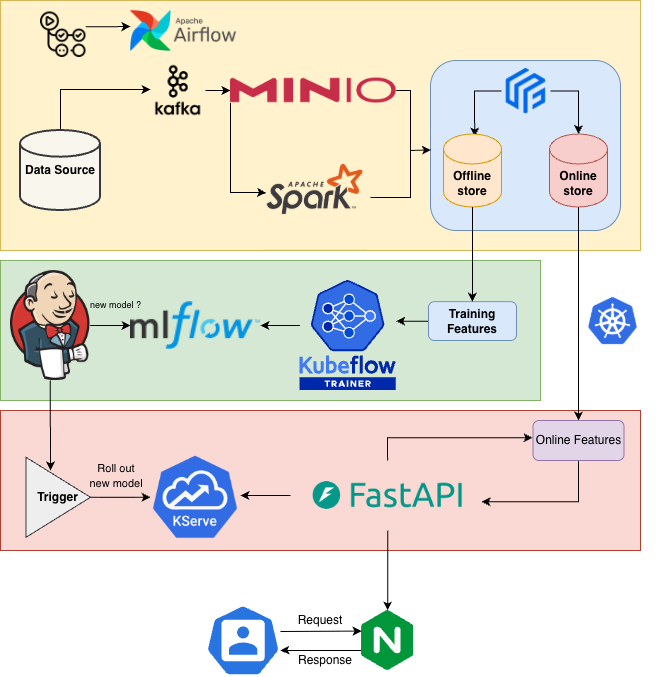
\includegraphics[width=\columnwidth]{figure/mlops_architecture.png}
  \caption{Proposed three-layer MLOps architecture for 
           cart-to-purchase conversion prediction.}
  \label{fig:mlops_architecture}
\end{figure}

The proposed MLOps pipeline is organized across three functional layers, as illustrated in Fig.~\ref{fig:mlops_architecture}.

\paragraph{Layer 1 --- Data Ingestion and Feature Engineering.}
Raw user interaction events are ingested via two parallel paths. Apache Airflow orchestrates scheduled batch processing for historical data, while Apache Kafka handles real-time event streaming for low-latency feature updates. Both paths persist data to MinIO, serving as the central S3-compatible object store. Apache Spark performs distributed feature computation over the raw event log, materializing processed features into a Feast feature store with dual backends: an \textit{Offline Store} for training-time batch retrieval and an \textit{Online Store} for sub-millisecond inference serving. Container orchestration across the entire layer is managed by Kubernetes.

\paragraph{Layer 2 --- Model Training and Registry.}
Training features are pulled from the Feast Offline Store into a Kubeflow Trainer pipeline, which executes distributed model training. All hyperparameters, evaluation metrics, and model artifacts are automatically versioned and registered in MLflow. A Jenkins CI/CD server continuously monitors the MLflow Model Registry for new model candidates and triggers the promotion workflow upon passing the configured deployment quality gate, defined as AUC-ROC $\geq 0.85$ 
and Accuracy $\geq 0.80$.

\paragraph{Layer 3 --- Serving and Inference.}
At inference time, online features are retrieved from the Feast 
Online Store and forwarded to a FastAPI inference service. Upon 
Jenkins promotion approval, KServe executes a zero-downtime rollout 
of the new model version to the serving endpoint. End-user prediction 
requests and responses are routed through an NGINX reverse proxy, 
which handles load balancing and SSL termination.

\subsection{TabICL Architecture}


The architecture of TabICLv2 is illustrated in Fig.~\ref{fig:tabiclv2}. 

Following TabICL, TabICLv2 chains column-wise embedding, row-wise interaction, and dataset-wise ICL, thus preserving the efficiency of TabICL with a runtime complexity of 
$\mathcal{O}(n^2 + nm^2)$ for tables with $n$ rows and $m$ columns. 
The subsequent sections elaborate on three architectural enhancements that we introduce in TabICLv2: \emph{repeated feature grouping}, \emph{target-aware embedding}, and \emph{query-aware scalable softmax}. For empirical validation and reproducibility, our framework utilizes an optimized implementation of the TabICLv2 architecture, structurally influenced by nanoTabPFN~\cite{Pfefferle2025NanoTabPFN}.

\paragraph{Repeated Feature Grouping.}
TabICL embeds each feature independently, which can lead to representation collapse when features share similar distributions. TabPFNv2 and TabPFN-2.5 mitigate this collapse by grouping multiple columns into single tokens, a strategy that simultaneously reduces the number of effective features to improve administrative efficiency; however, this reduction may precipitate the loss of fine-grained feature information. To circumvent this limitation, we introduce \emph{repeated feature grouping}, an algorithmic mechanism that maps each feature into multiple distinct groups via cyclic permutations, thereby preserving the dimensionality of the effective feature space. Specifically, for a table comprising $m$ columns, we synthesize $m$ overlapping groups, where the $j$-th group encapsulates columns at positions $(j, j+1, j+3) \bmod m$. Each group is subsequently encoded by a shared linear projection layer $\mathrm{Lin}: \mathbb{R}^3 \to \mathbb{R}^d$:
\begin{equation*}
	E_1[i,j] = \mathrm{Lin}\big(x_{i,j},\, x_{i, (j+1) \bmod m},\, x_{i, (j+3) \bmod m}\big).
\end{equation*}
The shift pattern $(0, 1, 3)$ ensures that for $\geq 7$ columns, no pair of columns appears together in more than one group.

\paragraph{Target-Aware Embedding.}
Empirical observations suggest that injecting target information early in the forward pass yields more robust representations. After repeated feature grouping yields the input data representation $E_1 \in \mathbb{R}^{n \times m \times d}$, we append target embeddings directly to each corresponding training token:
\begin{equation*}
	E_2[i,j] = E_1[i,j] + \mathrm{Embed_{\text{TAE}}}(y_i), \quad i \in \mathcal{D}_{\mathrm{train}},
\end{equation*}
where $\mathrm{Embed_{\text{TAE}}}$ is a linear layer for regression or a learnable lookup table for classification. Unlike TabPFNv2 appending the target as an additional column, we directly add target embeddings to all features. This also helps mitigate representation collapse because even when two features share similar distributions, their association with target values often differs across samples.

\name processes $E_2$ in three stages: (1) \emph{column-wise embedding} applies a set transformer $\TFcol$~\cite{set-transformer} to each column; (2) \emph{row-wise interaction} uses a transformer $\TFrow$ with [CLS] tokens to collapse feature embeddings per row into a single vector; (3) \emph{dataset-wise ICL} combines row embeddings with target embeddings and uses a transformer $\TFicl$ where test samples attend to training samples for prediction.

\paragraph{Query-Aware Scalable Softmax.}
To improve generalization to larger datasets, we extend Scalable Softmax, a temperature scaling method that sharpens attention distributions by rescaling queries before computing logits. Let $q_h = (q_{hi})$ be a query vector at head $h$ with head dimension indexed by $i$, and let $n$ be the size of the training set. SSMax rescales queries with a learnable per-head scalar $s_h$:
\begin{equation*}
    \tilde{q}_{hi} = q_{hi} \cdot s_h \log n~.
\end{equation*}

\begin{figure*}[!t]
\centering
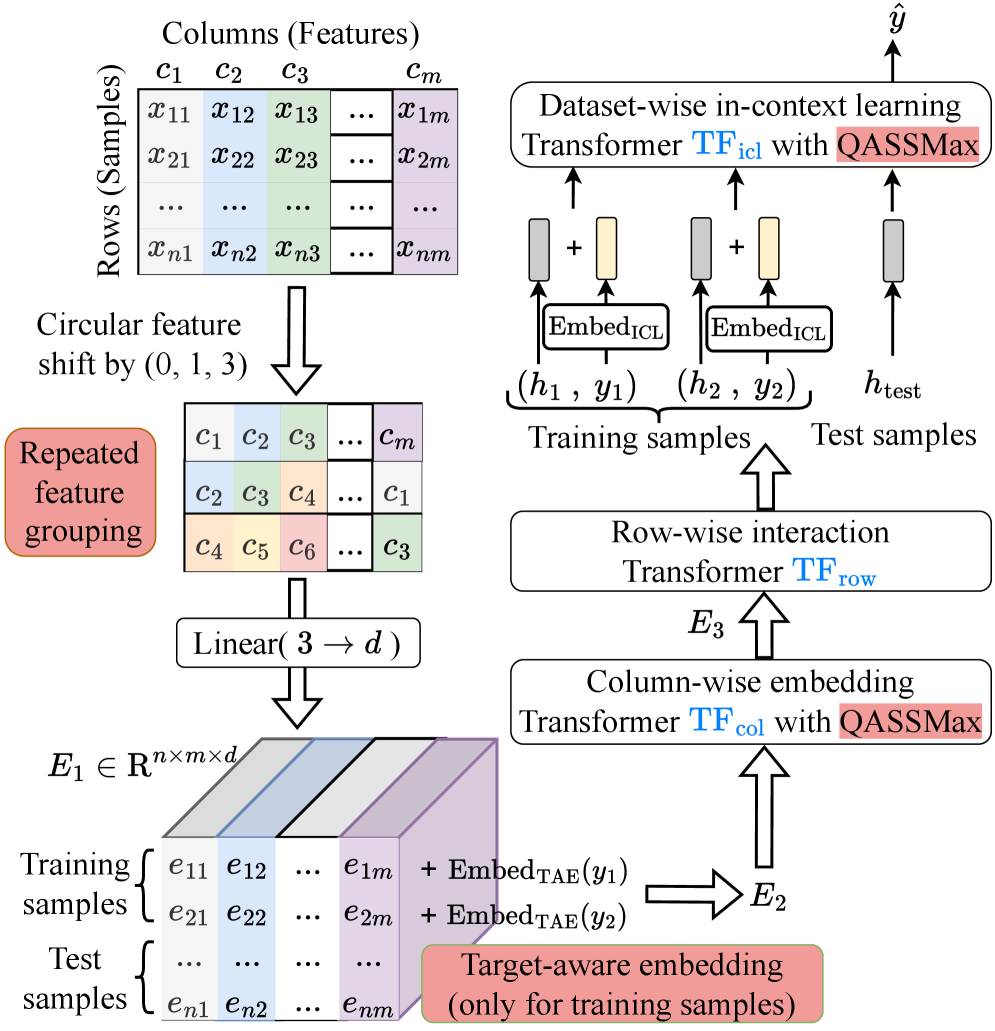
\includegraphics[width=0.82\textwidth]{figure/tabiclv2_architecture.png}
\caption{Architecture of TabICLv2, illustrating the three-stage pipeline: column-wise embedding (TF$_\text{col}$), row-wise interaction (TF$_\text{row}$), and dataset-wise in-context learning (TF$_\text{icl}$) with QASSMax attention.}
\label{fig:tabiclv2}
\end{figure*}

We propose query-aware scalable softmax (QASSMax), which rescales each query element as:
\begin{equation*}
	\tilde{q}_{hi} = q_{hi} \cdot \underbrace{\mathrm{MLP}_{\mathrm{base}}(\log n)_{hi}}_{\text{base scaling}} \cdot \underbrace{\big(1 + \tanh(\mathrm{MLP}_{\mathrm{gate}}(q_h)_i)\big)}_{\text{query-aware gating}}
\end{equation*}
where for $H$ attention heads, $\mathrm{MLP}_{\mathrm{base}}: \mathbb{R} \to \mathbb{R}^{H \times d_{\mathrm{head}}}$ and $\mathrm{MLP}_{\mathrm{gate}}: \mathbb{R}^{d_{\mathrm{head}}} \to \mathbb{R}^{d_{\mathrm{head}}}$ are two-layer MLPs with 64 hidden neurons and GELU activation.

\section{Experimental Design}

\subsection{Evaluation Protocol}

All experiments are conducted under identical data splits to ensure fair comparison. For each experiment, we perform 5-fold cross-validation with stratified splits to preserve class balance ($\approx$26\% positive rate). We report the following metrics:

\begin{itemize}
  \item \textbf{Accuracy}: Overall classification accuracy.
  \item \textbf{Precision}: Proportion of predicted purchases that are actual purchases.
  \item \textbf{Recall}: Proportion of actual purchases that are correctly identified.
  \item \textbf{F1-Score}: Harmonic mean of precision and recall.
  \item \textbf{AUC-ROC}: Area under the receiver operating characteristic curve.
  \item \textbf{Log Loss}: Binary cross-entropy loss, penalizing confident incorrect predictions.
  \item \textbf{Training Time}: Wall-clock seconds for training and inference.
\end{itemize}

For XGBoost, LightGBM, and CatBoost, all hyperparameters are optimized via Optuna Bayesian search over 50 trials. TabICL is applied with default settings and no hyperparameter tuning. The 75K sample dataset is used as the primary benchmark; scale analysis (50K--1M) and feature ablation experiments follow the same protocol.
Experiments are organized around three questions: (1) accuracy compared with strong GBDT baselines, (2) inference speed under large context sizes, and (3) robustness across datasets with different feature cardinality and class imbalance.

\section{Results and Discussion}

All experiments use 5-fold stratified cross-validation. We report mean $\pm$ standard deviation across folds.

\subsection{Benchmark Comparison (75K Samples)}

Table~\ref{tab:benchmark} compares all four models on the 75K sample benchmark with full feature engineering.

\begin{table*}[!htbp]
\centering
\caption{Model comparison on 75K samples (5-fold CV, mean$\pm$std). Bold indicates best.}
\label{tab:benchmark}
\renewcommand{\arraystretch}{1.1}
\begin{tabular}{lcccccc}
\toprule
Model & Acc. & Prec. & Recall & F1 & AUC & Time(s) \\
\midrule
XGBoost  & $.849{\pm}.003$ & $.718{\pm}.005$ & $.693{\pm}.004$ & $.705{\pm}.003$ & $.923{\pm}.002$ & $0.59{\pm}0.04$ \\
LightGBM & $.849{\pm}.003$ & $.718{\pm}.005$ & $.685{\pm}.005$ & $.701{\pm}.004$ & $.924{\pm}.002$ & $1.33{\pm}0.11$ \\
CatBoost & $.851{\pm}.002$ & $.\textbf{726}{\pm}.004$ & $.680{\pm}.005$ & $.702{\pm}.003$ & $.925{\pm}.002$ & $2.09{\pm}0.18$ \\
TabICL   & $.850{\pm}.003$ & $.723{\pm}.005$ & $.687{\pm}.004$ & $.704{\pm}.004$ & $\textbf{.925}{\pm}.002$ & $1.15{\pm}0.09$ \\
\bottomrule
\end{tabular}
\end{table*}

All models achieve comparable accuracy ($\approx$.850) and AUC ($\approx$.924). XGBoost leads in F1 ($.705$) via superior recall ($.693$); CatBoost achieves the highest precision ($.726$). TabICL matches the best GBDT in AUC ($.925$) without hyperparameter tuning, confirming that ICL can compete on large-scale e-commerce data.

\begin{figure}[t]
  \centering
  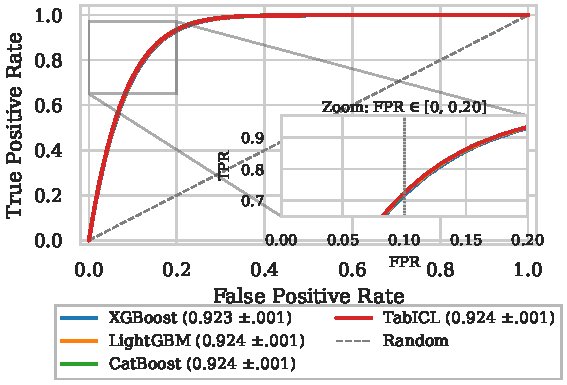
\includegraphics[width=\columnwidth]{figures/fig1_roc.pdf}
  \caption{ROC curves for all four models on 75K samples.}
  \label{fig:roc}
\end{figure}

\subsection{Scale Analysis}

Figure~\ref{fig:scale} and Table~\ref{tab:scale} compare XGBoost (with FE) and TabICL (without FE) across five training set sizes.

\begin{table*}[t]
\centering
\caption{XGBoost vs TabICL across training scales (5-fold CV). Best AUC per scale in bold.}
\label{tab:scale}
\renewcommand{\arraystretch}{1.1}
\begin{tabular}{lcccccc}
\toprule
 & \multicolumn{3}{c}{XGBoost (w/ FE)} & \multicolumn{3}{c}{TabICL (no FE)} \\
\cmidrule{2-7}
$n$ & Acc. & AUC & F1 & Acc. & AUC & F1 \\
\midrule
50K  & $.845{\pm}.004$ & $.917{\pm}.003$ & $.690{\pm}.005$ & $.848{\pm}.003$ & $.922{\pm}.003$ & $.701{\pm}.004$ \\
75K  & $.850{\pm}.003$ & $.923{\pm}.002$ & $.705{\pm}.003$ & $.850{\pm}.003$ & $\textbf{.925}{\pm}.002$ & $.704{\pm}.004$ \\
100K & $.853{\pm}.003$ & $.927{\pm}.002$ & $.712{\pm}.004$ & $.851{\pm}.003$ & $.924{\pm}.002$ & $.704{\pm}.003$ \\
500K & $.859{\pm}.003$ & $.930{\pm}.002$ & $.725{\pm}.003$ & $.848{\pm}.003$ & $.920{\pm}.003$ & $.697{\pm}.004$ \\
1M   & $.\textbf{863}{\pm}.002$ & $.\textbf{932}{\pm}.002$ & $.\textbf{740}{\pm}.003$ & $.846{\pm}.003$ & $.917{\pm}.003$ & $.692{\pm}.004$ \\
\bottomrule
\end{tabular}
\end{table*}

\begin{figure}[t]
  \centering
  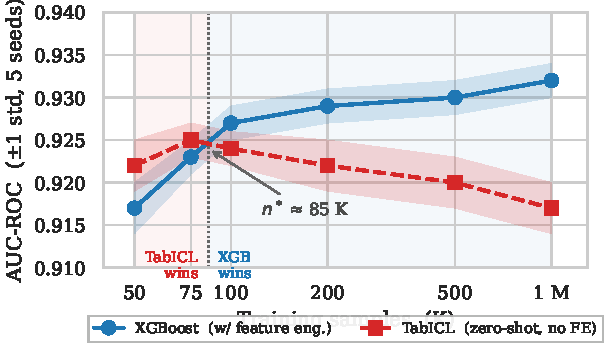
\includegraphics[width=0.75\columnwidth]{figures/fig2_scale.pdf}
  \caption{AUC-ROC versus training set size: XGBoost improves monotonically while TabICL peaks at 75K.}
  \label{fig:scale}
\end{figure}

XGBoost improves monotonically with scale ($+.015$ AUC from 50K to 1M), consistent with GBDT's ability to exploit larger datasets. TabICL peaks at 75K ($.925$) and degrades at larger scales ($.917$ at 1M), suggesting diminishing returns from ICL context beyond the model's effective range. The crossover occurs near 100K, after which GBDT dominates.


\subsection{Feature Ablation Study}

Figure~\ref{fig:ablation} and Table~\ref{tab:ablation} show the impact of removing engineered features (retaining only 4 raw features) on each model.

\begin{table*}[t]
\centering
\caption{Feature ablation on 75K samples (5-fold CV). $\Delta$ = Without FE $-$ With FE.}
\label{tab:ablation}
\renewcommand{\arraystretch}{1.1}
\begin{tabular}{lcccccc}
\toprule
 & \multicolumn{2}{c}{With FE} & \multicolumn{2}{c}{Without FE} & \multicolumn{2}{c}{$\Delta$} \\
\cmidrule{2-7}
Model & AUC & F1 & AUC & F1 & $\Delta$AUC & $\Delta$F1 \\
\midrule
XGBoost  & $.923{\pm}.002$ & $.705{\pm}.003$ & $.782{\pm}.006$ & $.558{\pm}.007$ & $-.141$ & $-.147$ \\
LightGBM & $.924{\pm}.002$ & $.701{\pm}.004$ & $.789{\pm}.005$ & $.565{\pm}.006$ & $-.135$ & $-.136$ \\
CatBoost & $.925{\pm}.002$ & $.702{\pm}.003$ & $.801{\pm}.005$ & $.578{\pm}.006$ & $-.124$ & $-.124$ \\
TabICL   & $\textbf{.925}{\pm}.002$ & $.704{\pm}.004$ & $.918{\pm}.002$ & $.698{\pm}.004$ & $-.007$ & $-.006$ \\
\bottomrule
\end{tabular}
\end{table*}

\begin{figure}[t]
  \centering
  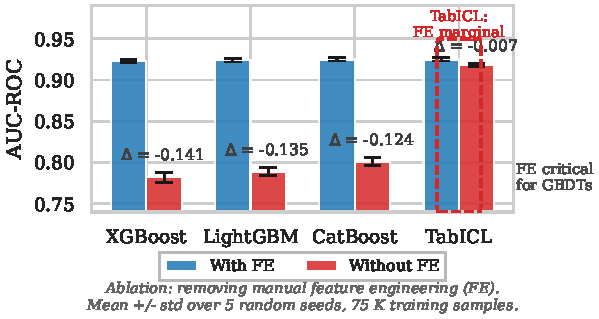
\includegraphics[width=\columnwidth]{figures/fig3_ablation.pdf}
  \caption{Feature ablation: GBDT degrades 12--14\% AUC without engineered features, while TabICL degrades only 0.8\%.}
  \label{fig:ablation}
\end{figure}



\subsection{Key Findings and Practical Implications}

Our empirical evaluation yields four main findings:

\begin{enumerate}
  \item \textbf{ICL achieves competitive accuracy without hyperparameter tuning.} TabICL matches the best GBDT in AUC on the 75K benchmark ($.925{\pm}.002$ vs~$.925{\pm}.002$) while requiring no task-specific optimization.
  \item \textbf{GBDT dominates at scale.} XGBoost AUC improves from $.917$ to $.932$ from 50K to 1M, while TabICL plateaus after 75K and degrades ($.917$ at 1M). GBDT is preferable for datasets $>$100K.
  \item \textbf{TabICL dramatically reduces feature dependency.} Without engineered features, GBDT degrades by $.124$--$.141$ AUC but TabICL by only $.007$. This makes TabICL attractive when FE resources are limited.
  \item \textbf{Inference latency favors XGBoost.} XGBoost trains in $0.59{\pm}0.04$s---$2\times$ faster than TabICL ($1.15{\pm}0.09$s) and $4\times$ faster than CatBoost ($2.09{\pm}0.18$s).
\end{enumerate}

\section{Limitations}

This study has several limitations that bound the generalizability of its findings. First, the evaluation is conducted on a single e-commerce dataset spanning seven months; results may differ on datasets with different temporal dynamics, user demographics, or product categories. Second, TabICL is evaluated in a single configuration with default hyperparameters, and systematic hyperparameter search may narrow the performance gap with XGBoost. Third, our MLOps deployment evaluation uses latency as the primary operational metric; throughput, memory footprint, and cost-per-inference---which are equally relevant in production environments---are not quantified. Fourth, this work does not address online learning or concept drift: both models are trained and evaluated in a fixed temporal split, and performance under distributional shift over time remains an open question. Finally, TabICLv2's GPU memory requirements, while lower than TabPFN, may still be prohibitive for resource-constrained deployments; the trade-off between model size and performance on e-commerce data warrants further investigation.

\section{Conclusion}

This paper presented a systematic empirical investigation contrasting tabular foundation models (specifically TabICL) against Gradient-Boosted Decision Trees for cart-to-purchase conversion prediction on a large-scale e-commerce behavioral dataset comprising over 285 million interaction events. Our results yield three main conclusions: (1) TabICL achieves competitive AUC-ROC ($.925$) with zero hyperparameter tuning, making it attractive for rapid prototyping; (2) XGBoost monotonically improves with scale up to $.932$ at 1M samples, maintaining a clear advantage for large-scale production systems; and (3) TabICL degrades by only $.007$ AUC without feature engineering versus $.124$--$.141$ for GBDT, revealing a fundamental difference in how the two paradigms exploit behavioral signals.

These findings have direct implications for practitioners: tabular foundation models like TabICL are a viable option when feature engineering resources are limited or when the deployment scenario demands minimal tuning overhead. However, for high-throughput, real-time serving environments with abundant training data, GBDT remains the more practical choice. Future work should investigate online adaptation strategies for TabICL to handle concept drift, explore hybrid architectures that combine the feature efficiency of ICL models with the scalability of gradient boosting, and extend evaluation to diverse e-commerce verticals and user segments.

\balance
\bibliographystyle{IEEEtran}
\bibliography{Bib_references}

\end{document}